\chapter{Zásuvný modul}
\label{4-plugin}

Čtvrtá kapitola popisuje vývoj zásuvného modulu a~rozebírá důležité části kódu.
Pro názornější popis jsou texty doplněny takzvanými pseudokódy,
schematickými přehledy nejdůležitějších částí kódového zpracování;
v~textové části se na takové části odkazuje označením příslušného pseudokódu a~řádku v~závorkách.  
Při samotné tvorbě kódu bylo vycházeno z~příručky \citep{cookbook}.

\section{Obsah CSV}
\label{obsah}

Vstupní soubor s~měřenými daty musí být tzv.~\zk{CSV}~(\textit{comma-separated values} - hodnoty oddělené
čárkami) soubor. Oddělování čárkami představuje pro čtení souboru zásuvným modulem zásadní podmínku.
Software v~měření radioaktivity (a~mnohdy i~jiných atributů) běžně používaný k~zápisu obvykle
%%% ML: vynechat "a" ?
produkuje právě soubory s~koncovkou~.\zk{CSV} s~nezbytnými i~doplňujícími atributy. Na pořadí
atributů nezáleží. 

Povinné části a~jejich označení v~hlavičce souboru: 
\begin{itemize}
	
%%% ML: {\tt Lat\_deg} ?
%%% ML: {\tt Lat\_deg}: Označuje ... ?
	\item {\tt Lat\_deg}: Sloupec {\tt Lat\_deg} obsahuje zeměpisnou šířku snímaného bodu na elipsoidu.
	Za referenční elipsoid, na němž se úloha vypočítává, byl zvolen nejběžněji užívaný
	elipsoid~\zk{WGS84}. 
	
	\item {\tt Lon\_deg}: Sloupec {\tt Lon\_deg} obsahuje zeměpisnou délku snímaného bodu na elipsoidu.
	Za referenční elipsoid, na němž se úloha vypočítává, byl zvolen nejběžněji užívaný
	elipsoid~\zk{WGS84}. 
	
	\item {\tt Gtm\_sec}: Čas měření ve vteřinách. Není důležité, jaký typ udávání času daný soubor
	podporuje (zda například počítá vteřiny od nějakého roku, nebo od začátku měření), počítá
	se s~rozestupy mezi jednotlivými údaji. 
	
	\item {\tt mereni}: {\tt mereni} obsahuje měřenou hodnotu (v~prezentovaném případě hodnotu
	radioaktivity, ale sloupec by mohl obsahovat jakoukoli jinou, i~nečíselnou hodnotu). Zásuvný modul
	posune body i~bez těchto hodnot, ale v~primárním určení, měření
	radioaktivity, by bez této hodnoty postrádal smysl.
	
%%% ML: je vzdy silne ?
	\item {\tt RECS}: Pod označením {\tt RECS} se skrývá číslo bodu. Tato položka nezbytná není, avšak
	číslování bodů zajišťuje lepší čitelnost dat, pročež je doporučováno užívat jej vždy. 

\end{itemize}

Soubor bývá doplněn o~data pro zásuvný modul zbytná, například číslo linie, souřadnice na jiném
referenčním tělese, nadmořskou výšku, jiný systém času nebo datace. 

  \begin{figure}[H]
   \centering
	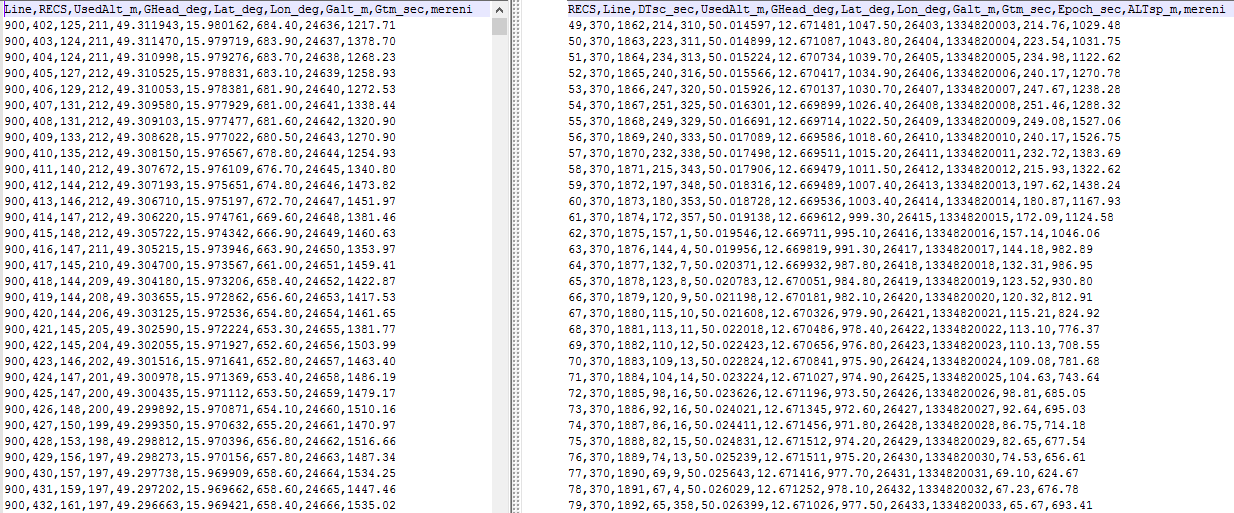
\includegraphics[scale=0.45]{./pictures/ukazka-vstup.png}
	\caption[Ukázka dvou typů vstupních souborů]{Ukázka dvou typů vstupních souborů
      \label{fig:ukazka-vstup}}
  \end{figure}

\section{Tělo zásuvného modulu}
\label{telo}

%%% ML: je opravdu Kosmogicky vhodne slovo s ohledem na vyznam teto vety?
Základ zásuvného modulu byl vytvořen ve volně šiřitelném mo\-dulu nazvaném Plugin
Builder\footnote{Dostupný na \textit{https://plugins.qgis.org/plugins/pluginbuilder/}}. Jedná se
%%% ML: napriklad ?
o~zásuvný modul vytvořený pro QGIS především (ale nikoli pouze) suitou kolem GeoApt LLC,
%%% ML: volne siritelny ?
skupi\-ny zaměřující se na volně šiřitelný \zk{GIS}. Plugin Builder na
základě uživatelem zadaných parametrů vytvoří základní skelet zásuvného modulu - ikonku, holobyt
grafického rozhraní, metadata, základní funkce (zapnout, vypnout) a~vazby zásuvného modulu. 

Fundamentální tělo zajišťující základní funkcionalitu zásuvného modulu je ulože\-no v~několika vzájemně
provázaných souborech: 
\begin{itemize}

%%% ML: {\tt \_\_init\_\_.py} ?
	\item {\tt \_\_init\_\_.py}: Základní inicializace zásuvného modulu. 

	\item {\tt plugin\_upload.py}: Zajišťuje všeobecnou dostupnost zásuvného modulu. 	

	\item {\tt position\_correction.py}: Implementuje zásuvný modul do prostředí QGIS. Načítá jeho ikonu,
	jmenuje a~aktivuje jej a~v~případě vypínání se stará o~jeho destrukci. Funkce \textit{run} jej váže
	s~position\_correction\_dockwidget.py. 
	
	\item {\tt position\_correction\_dockwidget.py}: Nejdůle\-žitěj\-ší
	ze základních souborů zá\-suvného modulu. Volání
	souboru {\tt position\_correction\_dockwidget\_base.ui}
	vytvoře\-ného v~prostředí Qt Designer
	zde vyvolává grafické uživatelské rozhraní. Zajišťuje
	také funkčnost ve\-škerých jeho částí a~celkové
%%% ML: maat?
%%%%%% OP: maat je počeštěný, původem staroegyptský pojem, cosi jako bohatší řád - označuje celkově
%%%%%%     všeobecný řád, harmonii, správné fungování, zákonnost, stabilní jednání, kde se vše chová dle
%%%%%%     očekávání, jinak dojde ke kolapsu (počítačová řeč - erroru). Nahradím to chudším "řádem"
	dodržování vnitřního řádu, od načítání cest vstupních
	a~výstupních dat přes jejich zobrazování a~stylování (volá
%%% ML: provedeni posunu ?
	{\tt show\_as\_layer.py}) až po samotné provedení posunu ({\tt move.py}).
	Na pozadí dochází ke kontrole vstupujících údajů, v~případě nesrovnalostí
%%% ML: veta o nehodach a psovi mi prijde prilis sroubovana...
	bude uživatel u\-pozorněn chybovým hlášením. Aby se zamezilo zbrklým nehodám, byly ke zpřístupnění
	tlačítek zabudovány podmínky - ke zpřístupnění tlačítka na zobrazení vstupního souboru musí být
	k~tomuto souboru definována cesta, taktéž k~samotnému posunu je třeba mít vyplněny všechny potřebné
	parametry. 
	
	\item {\tt show\_as\_layer.py}: Zobrazí soubor, an
	je předán jako jeden ze vstupních parame\-trů. Druhým
%%% ML: jako ze bych ty tridy implementoval sam od sebe, to nedava smysl
	vstupním parametrem je styl, jenž bude při zobrazování použit. Aby se zamezilo graviditě kódu
	a~obecné duplicitě kódu v~podhoubí prostředí QGIS, byly k~zobrazení užity interní objekty
	{\tt QgsVectorLayer} a~{\tt QgsMapLayerRegistry}. 

\end{itemize}

Toliko k~hrubému náčrtu fungování zásuvného modulu. Některé dílčí složky byly při představování
zane\-dbány, poněvadž nejsou k~pochopení fungování mo\-dulu nezbytné. Nyní se zvlášť podívejme na
soubory související se zkoumanou pro\-blematikou, tedy obsah move.py. 

%%% ML: krome pseudokodu (tam kde to pujde) doplnit obrazky
%%% zobrazujici danou situaci

\section{Posun o hodnoty}
\label{by_points}

  \begin{figure}[H]
   \centering
	
\includegraphics[scale=1]{./pictures/3-values-shift.png}
	\caption[Ukázka - Posun o 3 hodnoty]{Ukázka - Posun o 3 hodnoty (červeně vyznačeny posunuté body)
      \label{fig:values-shift}}
  \end{figure}

%%% ML: by_points() je metoda tridy Move. + dalsi vyskyty
Posun o~hodnoty se skrývá pod metodou {\tt by\_points} třídy {\tt Move}.
Zde nejprve proběhne analýza vstupních dat.
Analýza spočívá v~prohledání hlavičky souboru, je třeba zjistit polohu hledaných hodnot - sloupce
{\tt Lat\_deg} a~{\tt Lon\_deg}. 

Následně se čte vstupní soubor řádek po řádku a~postup posunu se liší na základě vstupní hodnoty posunu. 

\subsection{Posun o kladný počet hodnot}
\label{kladnehodnoty}

%%% ML: doplnit pseudokod nebo diagram
Jedná-li se o~číslo kladné, připojujeme k~informacím bodu \textit{n} souřadnice bodu
\textit{n+x}, kde \textit{x} představuje hodnotu, o~niž body posouváme. Toho dosáhneme tím, že
%%% ML: preformulovat
v~každé smyčce cyklu postupně načteme \textit{x} řádků, přičemž první z~těchto řádků vložíme do proměnné
(zbylé se nikam neukládají a~v~paměti tak nezůstávají - zůstává vždy pouze poslední čtený);
v~paměti tedy zbude první a~poslední z~čtených řádků
(pseudokód~\ref{alg:pseudokladnehodnoty}-1,~4). Hodnoty ze sloupců souřadnic posledního
načteného řádku vložíme do příslušných sloupců prvního čteného řádku
(pseudokód~\ref{alg:pseudokladnehodnoty}-5). Modifikovaný první
řádek se zapíše do výstupního souboru (pseudokód~\ref{alg:pseudokladnehodnoty}-6).
Načte se poloha konce prvního řádku (pseudokód~\ref{alg:pseudokladnehodnoty}-7) a~cyklus se může opakovat. 

%    \begin{figure}[h]
%    \centering
\begin{algorithm}
    \caption{Posun o kladné hodnoty}
    \label{alg:pseudokladnehodnoty}
    \begin{algorithmic}[1]

    \STATE{posunovanyradek=přečti první řádek}
    \WHILE{existuje posunovanyradek}
    \STATE{pozice=ulož pozici ve vstupním souboru}
    \STATE{přečti \textit{x} řádků}
    \STATE{vlož souřadnice posledního čteného řádku do posunovanyradek}
    \STATE{zapiš posunovanyradek}
    \STATE{seek(pozice)}
    \STATE{posunovanyradek=přečti řádek}
    \ENDWHILE
    \end{algorithmic}
\end{algorithm}
%    \caption{Pseudokód - Posun o kladné hodnoty}
%    \label{fig:pseudokladnehodnoty}
%    \end{figure}

%%% ML: uvazit pridani pseudokodu i pro ostatni algoritmu
\subsection{Posun o záporný počet hodnot}
\label{zapornehodnoty}

Jedná-li se o~číslo záporné, ještě před cyklem se provede odečtení \textit{x}~řádků,
kde \textit{x} je hodnota posunu; tyto řádky jsou zapsány do seznamu hodnot
(pseudokód~\ref{alg:pseudozapornehodnoty}-1).

Syžet cyklu následně probíhá
tím způsobem, že se z~tohoto seznamu odebírá první hodnota. Z~té jsou odečteny informace ze
sloupců příslušejících zeměpisným souřadnicím. Do dočasné proměnné je vložena poslední
hodnota seznamu (pseudokód~\ref{alg:pseudozapornehodnoty}-3)
a~její souřadnice jsou pře\-psány souřadnicemi výše zmiňovanými
(pseudokód~\ref{alg:pseudozapornehodnoty}-4). Modifikovaný řádek
se zapíše do výstupního souboru. Nyní je třeba doplnit seznam opět na \textit{x} hodnot, toho
se dosáhne čtením dalšího řádku ze vstupního souboru a~jeho vložením na konec seznamu
(pseudokód~\ref{alg:pseudozapornehodnoty}-8). Cyklus
se může opakovat. 

%    \begin{figure}[h]
 %   \centering
\begin{algorithm}
\caption{Posun o záporné hodnoty}
\label{alg:pseudozapornehodnoty}
    \begin{algorithmic}[1]
    \STATE{seznam=přečti \textit{x} řádků}
    \WHILE{existuje hodnota seznam[x]}
    \STATE{posunovanyradek=seznam[x]}
    \STATE{vlož souřadnice seznam[0] do posunovanyradek}
    \STATE{zapiš posunovanyradek}
%\algstore{myalg}
%\end{algorithmic}
%\end{algorithm}

%\begin{algorithm}                     
%\begin{algorithmic} [1]
%\algrestore{myalg}
    \STATE{vymaž seznam[0]}
    \STATE{seek(pozice)}
    \STATE{načti do seznamu další řádek}
    \ENDWHILE
    \end{algorithmic}
\end{algorithm}
%    \caption{Pseudokód - Posun o záporné hodnoty}
 %   \label{fig:pseudozapornehodnoty}
  %  \end{figure}

\subsection{Posun o nulový počet hodnot}
\label{nulovehodnoty}

Ve speciálním případě, kdy vstupuje do posunu o~hodnoty číslice~0,
dochází k~pouhé\-mu kopírování vstupního
souboru do souboru výstupního. Ovšem na žádný pád nemá v~takovém případě použití zásuvného modulu
odůvodnění. 

\section{Posun o konstantní vzdálenost}
\label{by_distance}

  \begin{figure}[H]
   \centering
	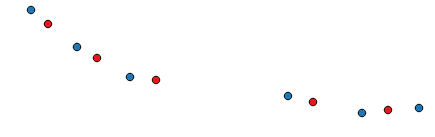
\includegraphics[scale=1]{./pictures/distance-shift.png}
	\caption[Ukázka - Posun o 9.823 metrů]{Ukázka - Posun o 9.823 metrů (červeně vyznačeny posunuté body)
      \label{fig:distance-shift}}
  \end{figure}

Posun o~konstantní vzdálenost je obsažen v~{\tt Move.by\_distance}. 

Na začátek funkce je třeba opět základní analýza vstupujícího souboru; její průběh je shodný
s~analýzou při posunu o~hodnoty (viz \ref{by_points}). 

Následně je třeba připravit si pole pro výpočty na elipsoidu. Redundance kódu není v~ničím
zájmu, pro potřeby elipsoidických operací tedy užíváme knihovnu
prostředí QGIS {\tt QgsDistanceArea}. Zde nastavíme
užitý referenční elipsoid \zk{WGS84}. 

Výpočet se opět liší dle povahy vstupující hodnoty posunu (kladná vzdálenost,
záporná, 0). Posledním krokem před rozlišením, kterou větev výpočtu volání funkce vyvolá, je nastavení
%%% ML: chybi obecne provazanost v textu, zde napr. viz kapitola 2.y
parametrů elipsoidu pro výpočet první geodetické úlohy (ta v~{\tt QgsDistanceArea} implemetována
není, a~je třeba ji řešit v~samotném kódu). Pro její obecný popis viz
\ref{prvnigu}, kódové zpracování bude popsáno později v~\ref{prvniguplugin} 

\subsection{Posun o kladnou vzdálenost}
\label{kladnavzdalenost}

Posunujeme-li body o~kladnou vzdálenost, na první pohled se nezdá, že by se v~algoritmu skrývaly
nějaké záludnosti. Na pohled druhý ano. 

Nejzásadnější problém se vynoří, snaží-li se uživatel posunout body o~vzdálenost větší, než
jaká se rozpíná mezi dvěma body. V~takovém případě je třeba v~momentě překročení zmiňované
vzdálenosti přepočítat trajektorii na novou dvojici bodů a~o~tuto hodnotu požadovanou
délku posunu snížit. 

Z~tohoto důvodu proběhne v~každém cyklu čtení \textit{x} řádků ve vnořeném cyklu \textit{while}
(pseudokód~\ref{alg:pseudokladnavzd-vnitrni}-4~až~11).
Tentokrát není \textit{x} daná hodnota, její velikost závisí na rozestupy mezi jednotlivými body.
V~každé smyčce vnitřního \textit{while} cyklu dojde k~výpočtu vzdálenosti mezi dvěma momentálně
načtenými body. Je-li vypočtená vzdálenost větší než délka posunu, cyklus skončí
(pseudokód~\ref{alg:pseudokladnavzd-vnitrni}-4). 
Avšak není-li, délka posunu se zkrátí o~vzdálenost mezi těmito body
(pseudokód~\ref{alg:pseudokladnavzd-vnitrni}-5) a~bodem~2 se nahradí bod~1
(pseudokód~\ref{alg:pseudokladnavzd-vnitrni}-6).
Vzápětí se čte další řádek představující nový bod~2
(pseudokód~\ref{alg:pseudokladnavzd-vnitrni}-7)
a~cyklus se opakuje. V~momentě, kdy
skončí, máme tedy novou dvojici bodů a~zbytek z posunu náležející na tento úsek.
%%% ML: probiha? poli?
Výpočet první geodetické úlohy tedy probíhá až v~takto předpřipraveném prostředí. 

%    \begin{figure}[h]
 %   \centering
\begin{algorithm}
\caption{Posun o kladnou vzdálenost, vnitřní cyklus}
\label{alg:pseudokladnavzd-vnitrni}
    \begin{algorithmic}[1]
    \STATE{radek2=radek}
    \STATE{vzdalenost=vzdálenost mezi posunovanyradek a radek}
    \STATE{delkaposunu=uživatelem volená hodnota posunu}
    \WHILE{delkaposunu>vzdalenost}
    \STATE{delkaposunu=delkaposunu-vzdalenost}
    \STATE{radek1=radek2}
    \STATE{radek2=přečti řádek}
    \IF{existuje radek2}
\algstore{myalg}
\end{algorithmic}
\end{algorithm}

\begin{algorithm}                     
\begin{algorithmic} [1]
\algrestore{myalg}
    \STATE{vzdalenost=vzdálenost mezi radek1 a radek2}
    \ENDIF
    \ENDWHILE
    \end{algorithmic}
\end{algorithm}
%    \caption{Pseudokód - Posun o kladnou vzdálenost, vnitřní cyklus}
 %   \label{fig:pseudokladnavzd-vnitrni}
  %  \end{figure}

Kromě zeměpisných souřadnic je ale třeba veškeré ostatní informace převzít z~prvního
čteného řádku (jediný, který kromě momentálního páru bodů zůstává v~paměti). Takto vytvořený
řádek se zapíše do výstupního souboru. Načte se poloha konce prvního čteného řádku
a~vnější cyklus se může opakovat. 

%    \begin{figure}[h]
 %   \centering
\begin{algorithm}
\caption{Posun o kladnou vzdálenost, vnější cyklus}
\label{alg:pseudokladnavzd-vnejsi}
    \begin{algorithmic}[1]
    \STATE{posunovanyradek=přečti řádek}
    \STATE{pozice=ulož pozici ve vstupním souboru}
    \WHILE{existuje posunovanyradek}
    \STATE{seek(pozice)}
    \STATE{radek=přečti řádek}
    \STATE{pozice=ulož pozici ve vstupním souboru}
    \IF{existuje radek}
    \STATE{vnitřní cyklus, viz pseudokód \ref{alg:pseudokladnavzd-vnitrni}}
%\algstore{myalg}
%\end{algorithmic}
%\end{algorithm}

%\begin{algorithm}                     
%\begin{algorithmic} [1]
%\algrestore{myalg}
	\STATE{výpočet první geodetické úlohy}
	\STATE{vlož vypočtené souřadnice do posunovanyradek}
    \STATE{zapiš posunovanyradek}
    \STATE{posunovanyradek=radek}
    \ENDIF
    \ENDWHILE
    \end{algorithmic}
\end{algorithm}
%    \caption{Pseudokód - Posun o kladnou vzdálenost, vnější cyklus}
 %   \label{fig:pseudokladnavzd-vnejsi}
  %  \end{figure}

\subsection{Posun o zápornou vzdálenost}
\label{zapornavzdalenost}

Vstupuje-li do posunu o~konstantní vzdálenost záporná hodnota, nabízí se možnost
využití kódu pro kladnou hodnotu, pouze s~inversně vyměněnými body. Opět bychom ale narazili
ve chvíli, kdy posun překračuje vzdálenost mezi dvěma body. 

Zde je zapotřebí jiného způsobu řešení problému. Tento úkol ztěžuje ještě fakt, že nechceme
zahltit paměť načítáním celého vstupního souboru, snažíme se tedy pracovat jen s~nutně
potřebnou dávkou řádků. 

Opět si vypomůžeme seznamem hodnot (řádků). Ponejprve byl vytvořen vstup\-ní seznam
na stejném principu, jako v~předchozím případě (porovnávání \textit{uražené} vzdálenosti se
vzdáleností mezi body), s~tím rozdílem, že tentokráte již použité body vkládáme do seznamu hodnot
(pseudokód~\ref{alg:pseudozapornavzd-vstup}-5~až~9).

%    \begin{figure}[h]
 %   \centering
\begin{algorithm}
\caption{Posun o zápornou vzdálenost, vytvoření vstupního seznamu}
\label{alg:pseudozapornavzd-vstup}
    \begin{algorithmic}[1]
    \STATE{seznam=přečti 2 řádky}
    \STATE{x=1}
    \STATE{delkaposunu=algolutní hodnota uživatelem volené hodnoty posunu}
    \STATE{urazenavzdalenost=vzdálenost mezi seznam[0] a seznam[1]}
    \WHILE{delkaposunu>urazenavzdalenost}
    \STATE{načti do seznamu další řádek}
    \STATE{x=x+1}
    \STATE{urazenavzdalenost=urazenavzdalenost+délka mezi seznam[x-1] a seznam[x]}
    \ENDWHILE
    \end{algorithmic}
\end{algorithm}
%    \caption{Pseudokód - Posun o zápornou vzdálenost, vytvoření vstupního seznamu}
 %   \label{fig:pseudozapornavzd-vstup}
  %  \end{figure}

Základní cyklus, jenž by se poznovu dal nazvat cyklem vnějším, se skládá ze dvou na sebe
navazujících cyklů vnitřních. 

První vnitřní cyklus slouží k~revizi, zda není seznam vstupující do výpočtu zbytečně obsáhlý.
Zjistí-li, že posun nepřekročí více než \textit{x} prvků
(pseudokód~\ref{alg:pseudozapornavzd-hlavnicyklus}-5), smaže redundantní prvky z~počátku seznamu (posouváme bod
z~konce seznamu). Na každý pád vstupuje do výpočtu seznam o~rozsahu právě onoho \textit{x}. 

Po dobrozdání výpočet vstupuje do cyklu spočívajícího ve výpočtu první geode\-tické úlohy.
Nadto do tohoto cyklu vstupují hodnoty kvůli posunu zpět v~reversním pořádku. Měl-li by
posun překročit vzdálenost mezi dvěma body, kvůli úspoře se výpočet přeskočí a~do pomocných
proměnných se zapíšou přímo souřadnice druhého z~bodů. 

Po smyčce, při kteréž již dojde k~výpočtu první geodetické úlohy
(dojde k~ní mezi prvními dvěma body seznamu - pseudokód~\ref{alg:pseudozapornavzd-hlavnicyklus}-10),
je proveden zápis do výstupního souboru - zapíše se poslední řádek ze seznamu se
zeměpisnými souřadnicemi přepsanými souřadnicemi vypočtenými (pseudokód~\ref{alg:pseudozapornavzd-hlavnicyklus}-11). 

\begin{algorithm}
\caption{Posun o zápornou vzdálenost, hlavní cyklus}
    \label{alg:pseudozapornavzd-hlavnicyklus}
%    \begin{figure}[h]
 %   \centering
    \begin{algorithmic}[1]
    \WHILE{poslední hodnota seznamu není prázdný řádek}
    \STATE{urazenavzdalenost=0}
\algstore{myalg}
\end{algorithmic}
\end{algorithm}

\begin{algorithm}                     
\begin{algorithmic} [1]
\algrestore{myalg}
    \FOR{i=obrácená řada od 1 do [velikost seznam]}
    \STATE{urazenavzdalenost=urazenavzdalenost+délka mezi seznam[i-1] a seznam[i]}
    \IF{delkaposunu<=urazenavzdalenost}
    \STATE{smaž body na pozici menší než i}
    \ENDIF
    \ENDFOR
    \STATE{posun=delkaposunu-(součet vzdáleností mezi body seznamu[1 až i])}
    \STATE{první geodetická úloha mezi seznam[1] a seznam[0], vzdálenost=posun}
    \STATE{vložíme vypočtené hodnoty do seznam[i] a zapíšeme jej}
    \STATE{načteme na konec seznamu další řádek}
    \ENDWHILE
    \end{algorithmic}
\end{algorithm}
%    \caption{Pseudokód - Posun o zápornou vzdálenost, hlavní cyklus}
 %   \label{fig:pseudozapornavzd-hlavnicyklus}
  %  \end{figure}

\subsection{Posun o nulovou vzdálenost}
\label{nulovavzdalenost}

Ježto by měl zásuvný modul fungovat i~při
operacích, které kterakkolivěk postrádají důvod k~jeho využití, byl do jeho
vnitřností implementován i~posun o~nulovou vzdálenost.
V~takovém případě se však vážně nejedná o~posun, nýbrž o~pouhé přepsání
neupravených hodnot ze vstupního souboru do souboru výstupního. 

\subsection{První geodetická úloha}
\label{prvniguplugin}

%%% ML: tady uz odkaz na teoretickou cast je, to je v poradku, v dalsim textu casto chybi
Velký problém při výpočtech na elipsoidu představuje první geodetická úloha. Ta byla popsána
již výše v~kapitole \ref{prvnigu}, nyní tedy pouze několiko poznámek k~jejímu kódovému zpracování. 

Samotný kód posunů se pro své značné množství nutných podmínek a~cyklů nevyznačuje
elegantní přehledností, pročež byl alespoň výpočet první geodetické úlohy vytržen jako zvláštní funkce.

Výpočet probíhá na základě iterací. Anžto byl jejich postup již výše popsán, jen zdůrazníme
některé části. Každá z~iterací zpřesňuje výpočet a~tyto iterace jsou prováděny do doby,
kdy přesnost dosáhne 0.0000000001~radiánu. 

Důležitým prvkem, který by neměl zůstat opomenut, jest vstupující azimut. Zde se musí pamatovat
na to, že azimut na elipsoidu se od azimutu na kouli či v~ro\-vině liší. Z~tohoto
důvodu byla využita funkce {\tt computeDistanceBearing} knihovny {\tt QgsDistanceArea}.

Nyní by bylo vhodné zdůvodnit právě tento druh výpočtu první geodetické úlohy a~nepoužití
složitější, arciť přesnější metody interpolace. 

Chtěli-li bychom vytvořit kód, který vykresluje trajektorii pravděpodobněji, mu\-sel by do
výpočtu vstupovat kompletní vstupní soubor; a~vzhledem k~tomu, že není ničím neobvyklým
soubor čítající mnoho přes 10000 záznamů o více než desítce sloupců, rozdíl v~systémové zátěži
by byl obrovský. 

Přesto byl tento návrh zpraco\-vá\-ní na poradě se Státním ústavem radiační ochra\-ny
vznesen. Po projednání bylo ze strany \zk{SÚRO} uvedeno, že vyhovuje námi momentálně
používaný způsob výpočtu; a~to nikolivěk pouze z~důvodu úspory systémových nároků, nýbrž především
z~toho důvodu, že výsledné zpřesnění souřadnic už by mělo na výsledky jejich práce
prakticky nulový vliv. 

\section{Posun o konstantní čas (proměnnou vzdálenost)}
\label{by_seconds}

  \begin{figure}[H]
   \centering
	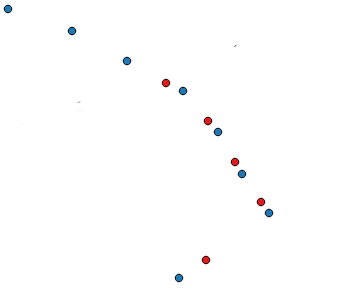
\includegraphics[scale=1]{./pictures/time-shift.png}
	\caption[Ukázka - Posun o 2.718 sekund]{Ukázka - Posun o 2.718 sekund (červeně vyznačeny posunuté body)
      \label{fig:time-shift}}
  \end{figure}

Velká část popisu kódu v~kapitole \ref{by_distance} se týká též posunu o~konstantní
čas - o~vzdále\-nost s~uvážením rychlosti. Odkazujeme se zde na základní přípravu hrací plochy,
analýzu, parametry elipsoidu a~vyvolání knihovny {\tt QgsDistanceArea}. Též výpočet první geodetické
úlohy se shoduje s výše popsanými postupy. Co se problémů jednotlivých
segmentů týče, dá se říci, že se dědí problémy posunu o~konstantní vzdálenost, pouze se k~nim
přidávají některé nové. 

Též základní fungování částí funkce se od těch popsaných výše příliš neliší; po\-psány tedy
budou pouze případné zásadnější odlišnosti. 

Nejočividnější rozdíl je pro veškeré posuny o~čas stejný - výpočet vzdálenosti,
o~niž se bod posouvá. Nejdříve je zapotřebí funkcí {\tt computeDistanceBearing}
vypočítat vzdálenost mezi dvojicí bodů. Vydělíme-li ji časovým úsekem, za který tuto vzdálenost
měřicí zařízení urazilo, získáme momentální rychlost. K~požadované délce posunu
se dostaneme již pouhým vynásobením této rychlosti uživatelem zadaným časovým úsekem. 

Z~uvedeného vyplývá, že je mezi dvojicí bodů předpokládán lineární pohyb. Taková idea vzešla
již od Státního ústavu radiační ochrany na základě toho, že vrtulník začíná měřit
až po jisté uražené vzdálenosti. V~tomto momentě již nabyl rychlost, kterou se snaží během
celého procesu měření konstantně udržovat. 

Zásadním problémem, který se při zpracování vynořil, je nejednotnost měření.
Ačkolivěk bývá zvykem měřit data po jedné sekundě, nedá se na takový postup spoléhat.
Používal-li by zásuvný modul cizinec, není vyloučené, že by v~jeho zemi bylo územ měřit
data po vteřinách třech nebo pěti. Je tedy třeba pracovat s~časovými značkami ze sloupce
{\tt Gtm\_sec} a~jejich rozdíly. Tím dochází k~zesložitění kódu, ale rovněž k~potřebnému
podchycení případných nesrovnalostí. 

Též je třeba ověřovat body vstupující do výpočtu první geodetické úlohy. Má-li měřicí zařízení
omezenou přesnost, může se stát, že budou mít dva po sobě měřené body zapsány stejné souřadnice.
Pokud by k~takové situaci došlo, je třeba se vyhnout výpočtu geodetické úlohy. Problém ani
tak nespočívá v~azimutu, jenž by mohl nabývat jakékoli hodnoty, nýbrž ve vzdálenosti.
Dělení nulou by vyvolávalo ve výpočtech chybu. Anžto vzdálenost mezi body jest nulová,
nastane zápis souřadnic jednoho z~bodů. 

\subsection{Posun o kladný časový úsek}
\label{kladnycas}

Při posunu o~kladný časový úsek je třeba vytvořit si pomocnou proměnnou, nazvěme ji zde \textit{x},
představující čas, o~který momentální bod posouváme. Ve chvíli vytvoření tedy bude \textit{x}
rovno uživatelem zadané hodnotě posunu. 

Před základním cyklem dojde k~odečtení a~uložení prvního řádku. Ten představuje posouvaný bod.
V~základním cyklu pak algoritmus čte další řádek. Ten představuje bod, k~němuž směřuje
trajektorie, po níž prvý bod posouváme. 

V~tomto vnějším cyklu opět pracuje cyklus vnitřní, v~kterémžto dochází k~porov\-ná\-vá\-ní našeho
\textit{x} s~dobou, za kterou měřicí zařízení urazilo vzdálenost mezi právě načtenou dvojicí bodů
(pseudokód~\ref{alg:pseudokladnycas}-10~až~15). 

Je-li \textit{x} menší než tato doba, proběhne výpočet první geodetické úlohy na trajektorii
a~s~uvážením rychlosti mezi těmito dvěma body (pseudokód~\ref{alg:pseudokladnycas}-11). 

Pokud se tyto hodnoty rovnají, jedná se o~podmínky pro výpočet ještě příznivější. Dojde k~pouhému
zápisu souřadnic druhého bodu do příslušných proměnných. V~ta\-ko\-vém
případě by se posun dal označit za posun o~hodnoty. 

Zákeřněji působí možnost, při níž je hodnota \textit{x} větší než doba mezi měřením dvou
bodů v~momentální paměti. Pak je zapotřebí dobu posunu \textit{x} zmenšit o~dobu, kterou
vrtulník mezi dvěma body urazil (pseudokód~\ref{alg:pseudokladnycas}-12),
druhý bod vložit do bodu prvního (pseudokód~\ref{alg:pseudokladnycas}-13) a~načíst
nový druhý bod (pseudokód~\ref{alg:pseudokladnycas}-14). Následně
se vnitřní cyklus zabývající se dobrozdáním ohledně hodnoty \textit{x} a~hodnoty
rozdílu časových značek mezi dvěma body v~paměti může opakovat. 

Poté, co jednou z~možných cest skončí vnitřní cyklus, dojde k~vložení nových souřadnic
(ať už vypočtených, nebo jen vyjmutých) do odpovídajících sloupců první\-ho čteného řádku.
Ten se zapíše do výstupního souboru (pseudokód~\ref{alg:pseudokladnycas}-16),
do proměnné \textit{x} se opět načte uživatelem volená
hodnota posunu, ve čtení se vyvolá pozice před započetím vnitřního cyklu, a~vnější cyklus se
opakuje s~řádky o~jeden posunutými (pseudokód~\ref{alg:pseudokladnycas}-4~až~19). 

\begin{algorithm}
    \caption{Posun o kladný čas}
    \label{alg:pseudokladnycas}
%    \begin{figure}[h]
 %   \centering
    \begin{algorithmic}[1]
    \STATE{posunovanyradek=přečti řádek}
    \STATE{radek1=posunovanyradek}
    \STATE{pozice=ulož pozici ve vstupním souboru}
    \WHILE{existuje posunovanyradek}
    \STATE{x=uživatelem zadaná hodnota posunu}
    \STATE{seek(pozice)}
    \STATE{nasledujiciradek=přečti řádek}
    \STATE{radek2=nasledujiciradek}
    \STATE{pozice=ulož pozici ve vstupním souboru}
    \WHILE{x>0}
     \STATE{vypočti první úlohu mezi radek1 a radek2}
     \STATE{x=x-(doba uplynulá mezi měřeními radek1 a radek2)}
\algstore{myalg}
\end{algorithmic}
\end{algorithm}

\begin{algorithm}                     
\begin{algorithmic} [1]
\algrestore{myalg}
     \STATE{radek1=radek2}
     \STATE{radek2=přečti řádek}
    \ENDWHILE
    \STATE{vlož vypočtené souřadnice do posunovanyradek a zapiš jej}
    \STATE{posunovanyradek=nasledujiciradek}
    \STATE{radek1=posunovanyradek}
    \ENDWHILE
    \end{algorithmic}
\end{algorithm}
 %   \caption{Pseudokód - Posun o kladný čas}
  %  \label{fig:pseudokladnycas}
   % \end{figure}

\subsection{Posun o záporný časový úsek}
\label{zapornycas}

Pro posun o~záporný časový úsek se jako ideální řešení opět zdálo využití seznamu řádků.
Tento seznam byl načten před samotným započetím vnějšího cyklu a~hodnoty do něj byly
přidávány do té doby, dokud součet rozdílů časových značek mezi jednotlivými body
nepřekročí uživatelem požadovanou hodnotu posunu (lépe řečeno její absolutní hodnotu,
poněvadž uživatel volí hodnotu zápornou). Tvoření seznamu naznačuje
pseudokód~\ref{alg:pseudokladnycas}-5~až~9). 

\begin{algorithm}
    \caption{Posun o záporný čas, vytvoření vstupního seznamu}
    \label{alg:pseudozapornycas-vstup}
%    \begin{figure}[h]
 %   \centering
    \begin{algorithmic}[1]
    \STATE{seznam=přečti 2 řádky}
    \STATE{x=1}
    \STATE{casuzivatel=absolutní hodnota uživatelem volené hodnoty posunu}
    \STATE{ubehlycas=rozdíl časových značek seznam[0] a seznam[1]}
    \WHILE{casuzivatel>ubehlycas}
    \STATE{načti do seznamu další řádek}
    \STATE{x=x+1}
    \STATE{ubehlycas=ubehlycas+rozdíl časových značek seznam[x] a seznam[x-1]}
    \ENDWHILE
    \end{algorithmic}
\end{algorithm}
%    \caption{Pseudokód - Posun o záporný čas, vytvoření vstupního seznamu}
 %   \label{fig:pseudozapornycas-vstup}
  %  \end{figure}

Seznam již vstupuje do vnějšího cyklu, jehož cílem je postupně projít celý vstupní
soubor a~posunout veškeré body. Tento cyklus se skládá ze dvou cyklů vnitřních. 

První vnitřní cyklus reviduje vstupující seznam hodnot. Zjišťuje, zda není přes\-příliš obsáhlý.
Kontrolu provádí na základě porovnávání součtu rozdílů časových značek s~uživatelem
voleným časovým posunem (pseudokód~\ref{alg:pseudozapornycas-hlavnicyklus}-3~až~8).
Narazí-li algoritmus na hodnoty, jež by nebyly při výpočtu využity
(pseudokód~\ref{alg:pseudozapornycas-hlavnicyklus}-5~až~7), ze seznamu je kvůli úspoře
paměti umaže (protože se nové hodnoty - posouvající se body - přidávají
na konec seznamu, nadbytečné hodnoty se nachází na jeho začátku). Tyto řádky totiž nebudou
třeba k~žádné z~následujících smyček. 

Druhý z~vnitřních cyklů se příliš neliší od toho popsaného v~kapitole \ref{zapornavzdalenost}.
Čte v~reversním pořadí seznam hodnot a~spočívá v~analýze vstupujících dat. Analýza
probíhá s~pomocnou proměnnou (v~textu si ji označme
\textit{x}), která představuje čas posunu od momentálního bodu. 

Pokud \textit{x} převyšuje dobu, za niž měřicí zařízení urazilo vzdálenost mezi dvěma načtenými
body, pouze se posuneme v~seznamu o úroveň níže (bod~1 se stane bodem 2 a~do nového
bodu 1 se vloží další řádek seznamu); \textit{x} se zmenší o~velikost zmiňovaného časového úseku. 

Rovnají-li se tyto dvě hodnoty, do paměti se uloží
souřadnice bodu 1 (bodu, k~němuž se počítá trajektorie). 

V~případě, že je absolutní hodnota \textit{x} menší než rozdíl časových značek, dochází
k~výpočtu první geodetické úlohy. Pseudokódy jsou jen schematické, poslední kroky
tedy shrnuje pseudokód (pseudokód~\ref{alg:pseudozapornycas-hlavnicyklus}-9~a~10)

Následuje chvíle pro již typickou koncovku vnějšího cyklu. Souřadnice z~paměti se vloží
do odpovídajících sloupců řádku s~posunovaným bodem a~ten se zapíše do
výstupního souboru (pseudokód~\ref{alg:pseudozapornycas-hlavnicyklus}-11).
Následně se na konec seznamu hodnot načte další řádek (nový posunovaný bod) a~\textit{x}
se nastaví na uživatelem volenou hodnotu posunu. Cyklus pokračuje další smyčkou. 

\begin{algorithm}
    \caption{Pseudokód - Posun o záporný čas, hlavní cyklus}
    \label{alg:pseudozapornycas-hlavnicyklus}
%    \begin{figure}[h]
 %   \centering
    \begin{algorithmic}[1]
    \WHILE{poslední hodnota seznamu není prázdný řádek}
    \STATE{ubehlycas=0}
    \FOR{i=obrácená řada od 1 do [velikost seznam]}
    \STATE{ubehlycas=rozdíl časových značek seznam[0] a seznam[1]}
    \IF{casuzivatel<=ubehlycas}
    \STATE{smaž body na pozici menší než i}
    \ENDIF
    \ENDFOR
    \STATE{casposunu=casuzivatel-(rozdíl časových značek seznam[i] a seznam[1])}
\algstore{myalg}
\end{algorithmic}
\end{algorithm}

\begin{algorithm}                     
\begin{algorithmic} [1]
\algrestore{myalg}
    \STATE{první geodetická úloha mezi seznam[1] a seznam[0], vzdálenost vypočtená z casposunu}
    \STATE{vložíme vypočtené hodnoty do seznam[velikost seznam-1] a zapíšeme jej}
    \STATE{načteme na konec seznamu další řádek}
    \ENDWHILE
    \end{algorithmic}
\end{algorithm}
%    \caption{Pseudokód - Posun o záporný čas, hlavní cyklus}
 %   \label{fig:pseudozapornycas-hlavnicyklus}
  %  \end{figure}

\subsection{Posun o nulový časový úsek}
\label{nulovycas}

Byť živou věcí neexistuje důvod k~použití zásuvného modulu za účelem takové ope\-race,
dovede si zásuvný modul poradit i~s~případem posunu o~0~sekund. Abychom se vyhnuli
naprosto zbytečné zátěži ve formě počítání nulových posunů, poznovu tato část kódu
funguje jen jako kopírování vstupního souboru do souboru výstupního. 

\section{Licence}
\label{licence}

Nebtě byl zásuvný modul vytvořen pro QGIS a~využívá jeho knihoven, dědí jeho licenci: GNU General Public
License~(\zk{GPL}). 

Jde o~\textit{copyleftovou} (odvozené dílo musí být dostupné pod stejnou licencí)
licenci. Ve své podstatě zde nejde o~omezování svobody, alebrž právě o~její dodržování - zajišťuje,
aby prvotně svobodný software tuto svobodu modifikacemi či přidáváním neztratil. 



